\author{Lucas Månsson}
\documentclass[a4paper,12pt]{article}
\usepackage[utf8]{inputenc}
\usepackage{amsmath, amssymb}
\usepackage{float}
\usepackage{parskip}
\usepackage{graphicx} 

\graphicspath{ {images/} }

\title{Flerdimensionell analys \\ Formelblad och anteckningar LP1 2025}
\date{}

\begin{document}
\maketitle

\section{Kapitel 1: Grundläggande begrepp}

\subsection{Mängder och tallinjen $\mathbb{R}$}
Snitt, union och differens:
\begin{figure}[H]
  \centering
  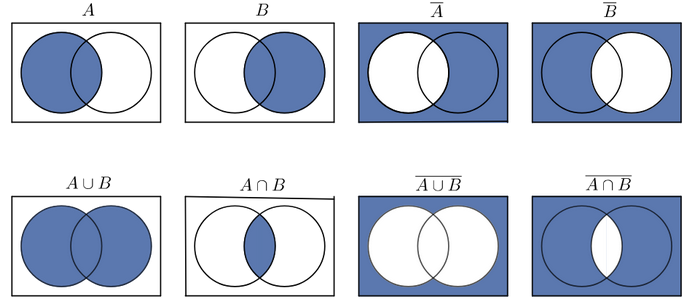
\includegraphics[width=1\textwidth]{snittuniondifferens.png}
  \caption{}
\end{figure}

\[
A \cup B, \quad A \cap B, \quad A \setminus B
\]

Absolutbelopp:

\[
    |ab| = |a||b|, \quad |\frac{a}{b}| = \frac{|a|}{|b|} \quad |a+b| \leq |a| + |b|
\]

\subsection{Planet $\mathbb{R}^2$ och rummet $\mathbb{R}^3$}
Avståndsformel.  
\[
    d = \sqrt{(x_1 - x_2)^2 + (y_1 - y_2)^2}
\]

\subsubsection*{Mängder i planet och rummet}
\textbf{Omgivning:}  
Med en omgivning av punkten $(a, b)$ i planet menar vi alla punkter i en cirkelskiva kring denna. Detta kan uttryckas:

\[
|(x,y) - (a,b)| < d
\]

Notera att den stränga olikheten ovan innebär att punkterna på själva cirkeln inte ingår i omgivningen.

\textbf{Öppen och sluten mängd.}

\subsection{Begrepp och metoder från linjär algebra}

\subsubsection*{Vektorer}
\[
u + v = (a_1,b_1) + (a_2,b_2) = (a_1+a_2, \, b_1+b_2)
\]
\[
u - v = (a_1,b_1) - (a_2,b_2) = (a_1-a_2, \, b_1-b_2)
\]
\[
\lambda u = \lambda (a_1, b_1) = (\lambda a_1, \lambda b_1)
\]
\[
|u+v| \leq |u| + |v|
\]

\subsubsection*{Skalärprodukt och vektorprodukt}
Skalärprodukt:
\[
u \cdot v = |u||v|\cos\theta
\]
\[
u \cdot v = (a_1, b_1)\cdot(a_2, b_2) = a_1a_2 + b_1b_2
\]

\subsubsection*{Ortogonal projektion}
En ortogonal projektion kan beräknas med projektionsformeln.
\begin{figure}[H]
  \centering
  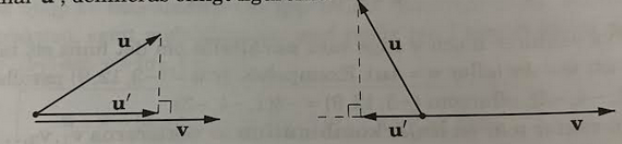
\includegraphics[width=1\textwidth]{ortogonalprojektion.png}
  \caption{}
\end{figure}
\[
    \mathbf{u'} =  \frac{\mathbf{u} \cdot \mathbf{v}}{\|\mathbf{v}\|^2} \mathbf{v}
\]

\subsubsection*{Linjer}
Vi kan beskriva en linje i planet om vi känner till en punkt $P$ på linjen och en riktningsvektor $v$ som anger dess riktning.  

Om $P=(x_0, y_0)$ och $v = (v_1, v_2)$ så blir linjens ekvation i parameterform:
\[
(x, y) = (x_0, y_0) + t(v_1, v_2)
\]

\textbf{Normalvektor:}  
Varje linje i planet kan beskrivas på normalform:
\[
ax + by + c = 0
\]

Om vi plockar ut koefficienterna framför $x$ och $y$ och bildar vektorn $n = (a,b)$ blir $n$ vinkelrät mot linjen.  

Givet en punkt $P=(x_0,y_0)$ och normalvektor $n=(a,b)$:
\[
a(x - x_0) + b(y - y_0) = 0
\]

\subsubsection*{Plan}
Med hjälp av en punkt och två icke-parallella riktningsvektorer kan man få ett plan på parameterform i rummet.

\subsubsection*{Matriser och determinanter}

\subsection{Rummet $\mathbb{R}^n$}


\section{Kapitel 2: Analytisk geometri}

\subsection{Geometri i $\mathbb{R}^2$}
\subsubsection*{Sammanfattning av första- och andragradskurvor:}
\textbf{Rät linje:}

\begin{figure}[H]
  \centering
  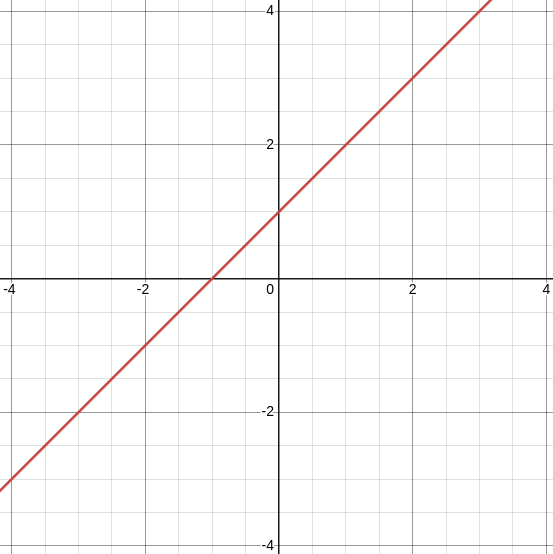
\includegraphics[width=0.25\textwidth]{ratlinje.png}
  \caption{}
\end{figure}
\[
ax + by + c = 0
\]

Parabel:
\begin{figure}[H]
  \centering
  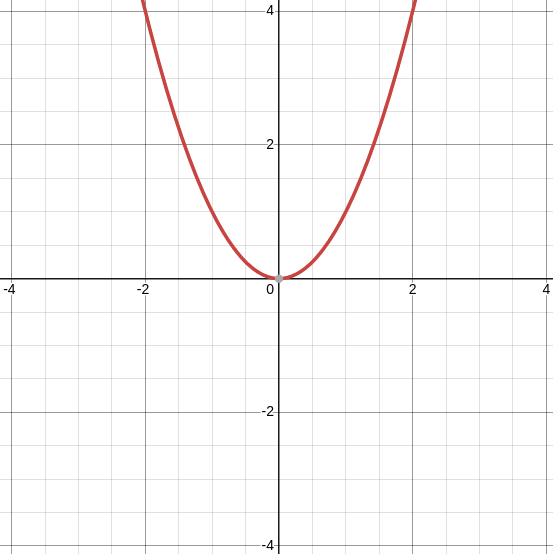
\includegraphics[width=0.25\textwidth]{parabel.png}
  \caption{}
\end{figure}
\[
y = ax^2
\]

Cirkel:
\begin{figure}[H]
  \centering
  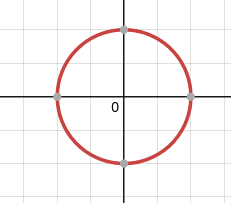
\includegraphics[width=0.25\textwidth]{cirkel.png}
  \caption{}
\end{figure}
\[
x^2 + y^2 = r^2
\]

Ellips
\begin{figure}[H]
  \centering
  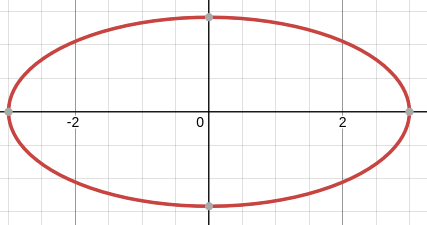
\includegraphics[width=0.25\textwidth]{ellips.png}
  \caption{}
\end{figure}
\[
\frac{x^2}{a^2} + \frac{y^2}{b^2} = 1, \quad \text{asymptoter: } y = \pm \frac{b}{a}x
\]

Hyperbel
\begin{figure}[H]
  \centering
  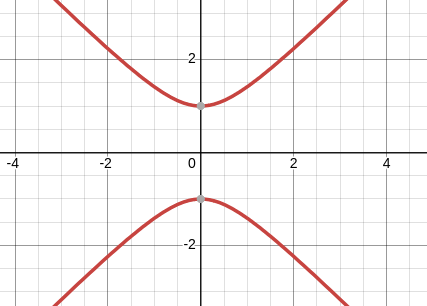
\includegraphics[width=0.25\textwidth]{hyperbel.png}
  \caption{}
\end{figure}
\[
\frac{x^2}{a^2} - \frac{y^2}{b^2} = 1, \quad \text{asymptoter: } y = \pm \frac{b}{a}x
\]
För en hyperbel med höger-vänster öppen:
\[
\frac{y^2}{b^2} - \frac{x^2}{a^2} = 1
\]

\subsection{Geometri i $\mathbb{R}^3$}
\subsubsection*{Sammanfattning av första- och andragradskurvor}

\textbf{Plan}
\[
ax + by + cz + d = 0
\]
\begin{figure}[H]
  \centering
  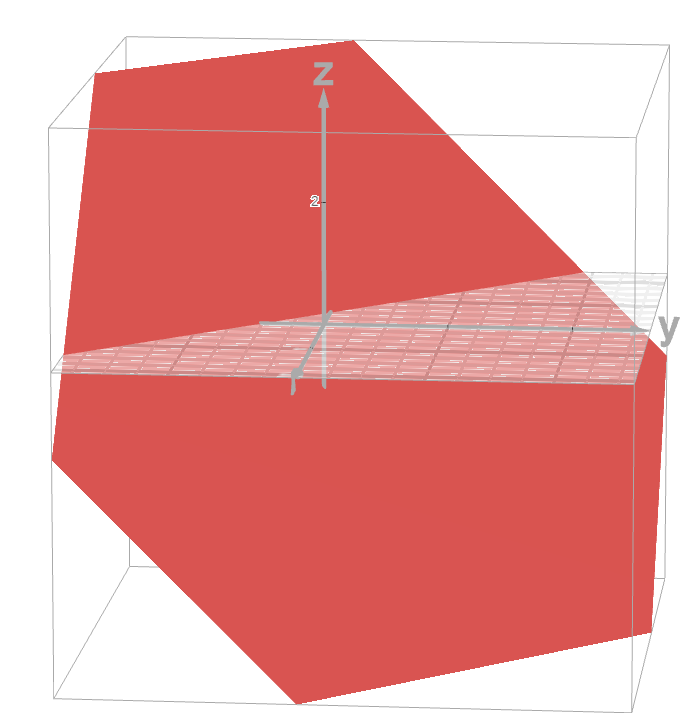
\includegraphics[width=0.25\textwidth]{plan.png}
  \caption{}
\end{figure}

\textbf{Paraboloid}
\[
z = \frac{x^2}{a^2} + \frac{y^2}{b^2}
\]
\begin{figure}[H]
  \centering
  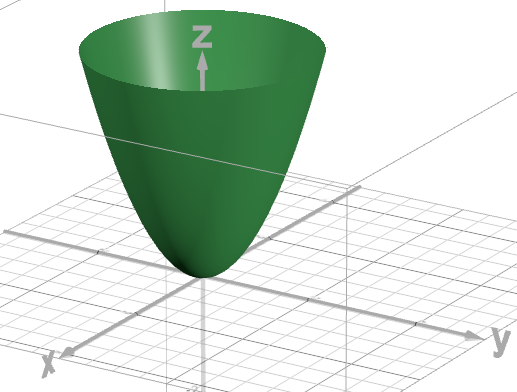
\includegraphics[width=0.25\textwidth]{paraboloid.png}
  \caption{}
\end{figure}

\textbf{Kon}
\[
z^2 = \frac{x^2}{a^2} + \frac{y^2}{b^2}
\]
\begin{figure}[H]
  \centering
  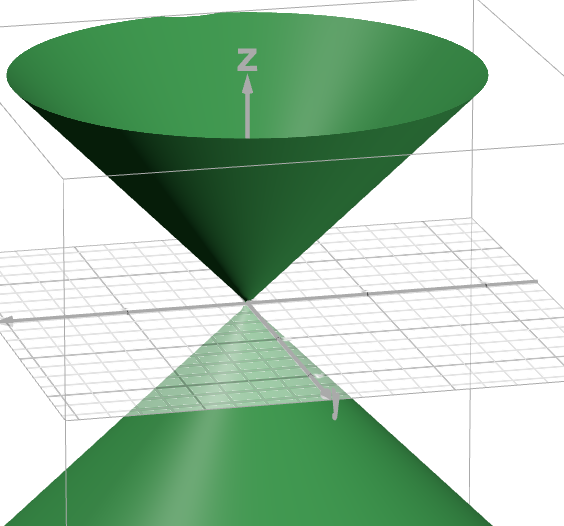
\includegraphics[width=0.25\textwidth]{kon.png}
  \caption{}
\end{figure}

\textbf{Sfär}
\[
x^2 + y^2 + z^2 = r^2
\]
\begin{figure}[H]
  \centering
  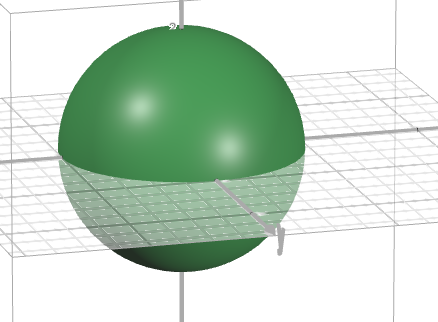
\includegraphics[width=0.25\textwidth]{sfar.png}
  \caption{}
\end{figure}

\textbf{Ellipsoid}
\[
\frac{x^2}{a^2} + \frac{y^2}{b^2} + \frac{z^2}{c^2} = 1
\]
\begin{figure}[H]
  \centering
  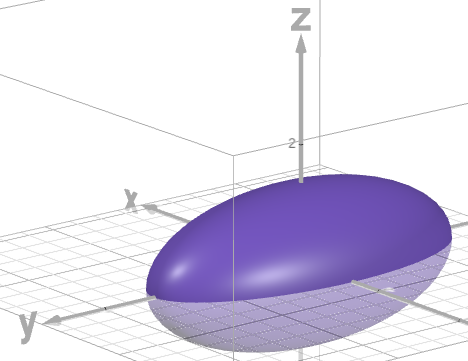
\includegraphics[width=0.25\textwidth]{ellipsoid.png}
  \caption{}
\end{figure}

\textbf{Hyperbolisk paraboloid}
\[
z = \frac{x^2}{a^2} - \frac{y^2}{b^2}
\]
\begin{figure}[H]
  \centering
  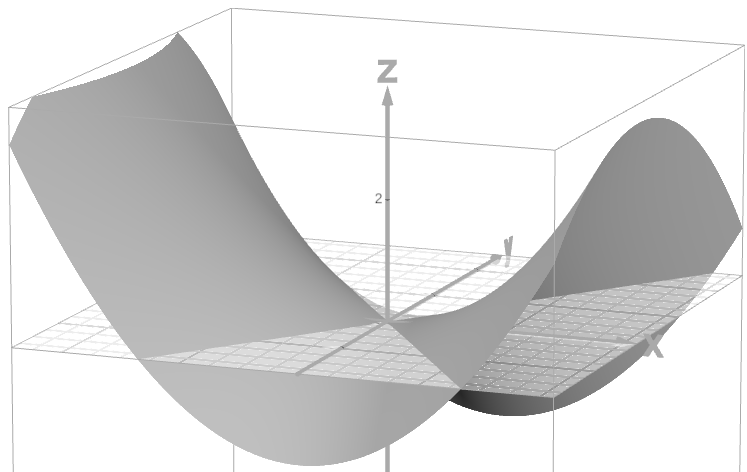
\includegraphics[width=0.25\textwidth]{hyperboliskparaboloid.png}
  \caption{}
\end{figure}

\textbf{Hyperboloid (enmantlad)}
\[
\frac{x^2}{a^2} + \frac{y^2}{b^2} - \frac{z^2}{c^2} = 1
\]
\begin{figure}[H]
  \centering
  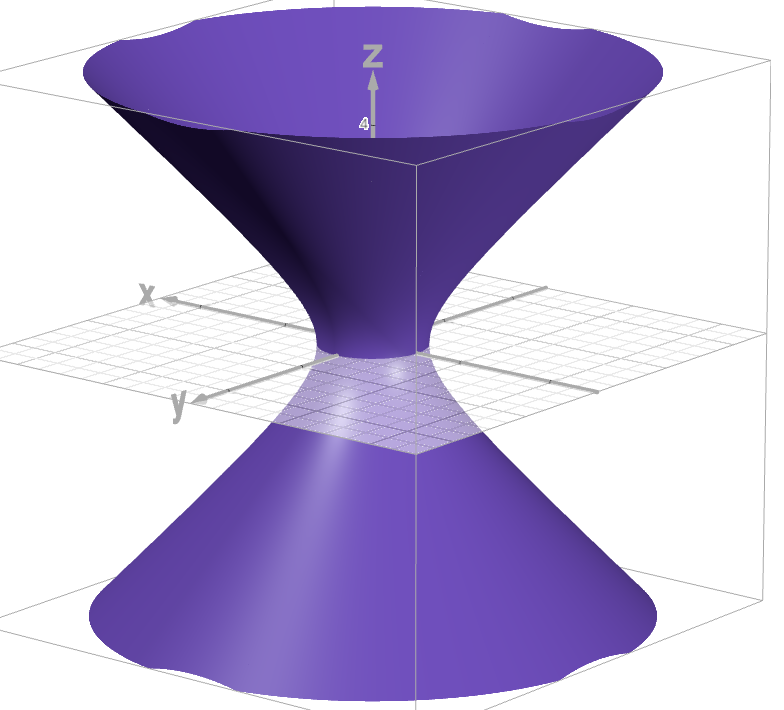
\includegraphics[width=0.25\textwidth]{enmantladhyperboloid.png}
  \caption{}
\end{figure}

\textbf{Hyperboloid (tvåmantlad)}
\[
-\frac{x^2}{a^2} - \frac{y^2}{b^2} + \frac{z^2}{c^2} = 1
\]
\begin{figure}[H]
  \centering
  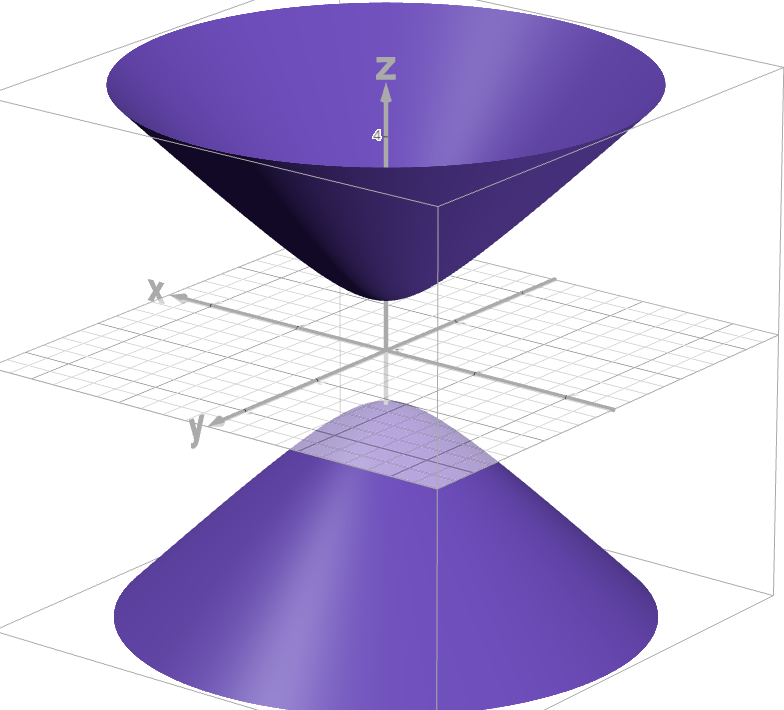
\includegraphics[width=0.25\textwidth]{tvamantladhyperboloid.png}
  \caption{}
\end{figure}

\subsection{Polära och rympolära koordinater}
\subsubsection*{Polära koordinater}
En punkt $P$ i planet med rätvinkliga koordinater $(x, y)$, 
kan också beskrivas med avståndet r från origo tillsammans med vinkel $\varphi$ mot positiva x-axeln.
$P$ har då polära koordinaterna $(r, \varphi)$. 
\begin{figure}[H]
  \centering
  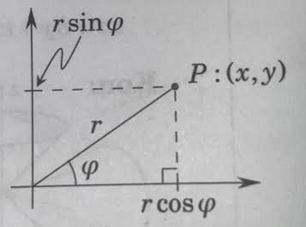
\includegraphics[width=0.25\textwidth]{polarakoordinater.png}
  \caption{}
\end{figure}
\[
\begin{cases}
x = r \sin \varphi, \\
y = r \sin \varphi 
\end{cases}
\]
I de fall vi har annan medelpunkt än origo, ex. $(x_0, y_0)$:
\[
\begin{cases}
x = x_0 + r \sin \varphi, \\
y = y_0 + r \sin \varphi 
\end{cases}
\]
Om vi vill beskriva en ellipsskiva, snarare än bara en ellips:
\[
\begin{cases}
x = x_0 + a r \sin \varphi, \\
y = y_0 + a r \sin \varphi 
\end{cases}
\]

\subsubsection*{Cylindriska och rymdpolära koordinater}
Cylindriska koordinater:
\begin{figure}[H]
  \centering
  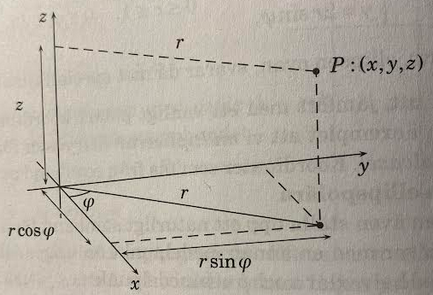
\includegraphics[width=0.5\textwidth]{cylindriskakoordinater.png}
  \caption{}
\end{figure}
\[
\begin{cases}
x = r \sin \varphi, \\
y = r \sin \varphi, \\
z = z
\end{cases}
\]

En annan koordinat än $z$ kan vara oförändrad.

Rymdpolära koordinater:
\begin{figure}[H]
  \centering
  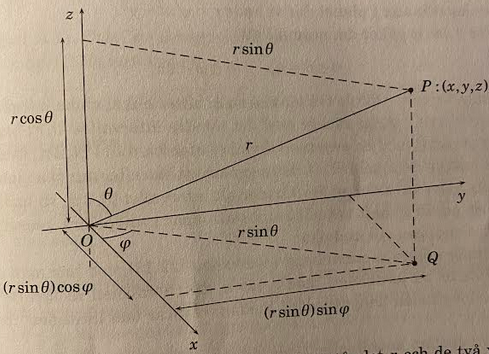
\includegraphics[width=0.5\textwidth]{rymdpolarakoordinater.png}
  \caption{}
\end{figure}
\[
\begin{cases}
x = r \sin \theta \cos \varphi, \\
y = r \sin \theta \sin \varphi, \\
z = r \cos \theta
\end{cases}
\]

\section{Kapitel 3: Funktioner}

\subsection{Reellvärda funktioner}
En reellvärd funktion är av typen
\[
\mathbb{R}^n \to \mathbb{R}
\]
dvs. en funktion av $n$ variabler där varje funktionsvärde är reellt.

\subsubsection*{Funktioner av typen $\mathbb{R}^2 \to \mathbb{R}$}
En funktion $f$ av två variabler består av en definitionsmängd $D_f \subseteq \mathbb{R}^2$ och en avbildningsregel:
\[
(x,y) \in D_f \mapsto f(x,y) \in \mathbb{R}
\]

\subsubsection*{Nivåkurvor och nivåytor}
En nivåkurva består av samtliga punkter i $xy$-planet som ger samma funktionsvärde. 
Låt f vara en funktion av två variabler, och C, en konstant. Mängden i xy - planet som ges av ekvationen:
\[
    f(x,y) = C
\]
kallas en \textbf{nivåkurva} till f. Konstanten C motsvarar således “höjden över xy-planet”.
\begin{figure}[H]
  \centering
  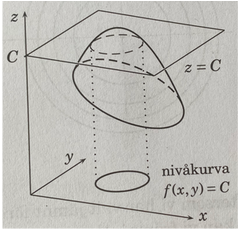
\includegraphics[width=0.25\textwidth]{nivakurva.png}
  \caption{}
\end{figure}

\subsection{Vektorvärda funktioner}
En funktion av typen $f: \mathbb{R}^n \to \mathbb{R}^p$, där $p \ge 2$, kallas \textbf{vektorvärd}.
eftersom funktionsvärdena då är vektorer.
\subsubsection*{Funktioner av typen $\mathbb{R} \to \mathbb{R}^2$ och $\mathbb{R} \to \mathbb{R}^3$ (kurvor)}
\[
    \textbf{r}(t) = (x(t), y(t))
\]
\[
    \textbf{r}(t) = (x(t), y(t), z(t))
\]

\subsubsection*{Funktioner av typen $\mathbb{R}^2 \to \mathbb{R}^3$ (ytor)}
\[
    \textbf{r}(s, t) = (x(s, t), y(s, t), z(s, t))
\]

\subsubsection*{Funktioner av typen $\mathbb{R}^2 \to \mathbb{R}^2$ och $\mathbb{R}^3 \to \mathbb{R}^3$ (koordinatbyten)}
(fyll i senare)

\subsubsection*{Funktioner av typen $\mathbb{R}^2 \to \mathbb{R}^2$ och $\mathbb{R}^3 \to \mathbb{R}^3$ (vektorfält)}
(fyll i senare)

\subsection{Sammansättning av funktioner}
\[
    (f \circ g)(x) = f(g(x))
\]

\subsection{Gränsvärden och kontinuitet}
\subsubsection*{Definition av gränsvärden då $(x, y) \to (a, b)}
Vi säger att $f(x, y)$ har gränsvärdet $A$ då $(x, y) \to (a, b)$, och skriver
\[
    \lim_{(x, y) \to (a, b)}f(x, y) = A,
\]

\subsubsection*{Beräkning av gränsvärden då $(x, y) \to (a, b)}
I envariabelfallet finns det endast två sätt att närma sig en punkt. Med två variabler finns det oändligt många.Ett sätt att hantera är att uttrycka punkterna i polära koordinater.
\[
\begin{cases}
x = r \sin \varphi, \\
y = r \sin \varphi 
\end{cases}
\]

Tillvägagångssätt:
\begin{itemize}
    \item Gör en kvalificerad gissning av vad gränsvärdet bör vara
    \item Bilda absolutbeloppet $|f(x, y) - A|$, byt till polära koordinater, och försök att göra $|f(x,y) - A|$ oberoende av $\varphi$ genom en lämplig uppskattning uppåt.
    \item Visa att denna uppskattning går mot 0 då $r \to 0$.
\end{itemize}

\subsubsection*{Beräkning av gränsvärden då $|(x, y)| \to \infty}
(Fyll i vid behov)

\subsubsection*{Gränsvärden för allmänna funktioner $\mathbb{R}^n \to \mathbb{R}^p$}
(Fyll i vid behov)

\subsubsection*{Kontinuitet}
Låt funktionen $f$ vara en funktion av typen $\mathbb{R}^2 \to \mathbb{R}^$ som är definerad i punkten $(a, b)$. Om det gäller att
\[
    \lim_{(x,y) \to (a, b)}f(x, y) = f(a, b)
\] 
är $f$ kontinuerlig i $(a, b)$.
Antag att den reellvärda funktionen $f(x, y)$ är kontinuerlig på den slutna begränsade (dvs. kompakta) mängden D i plaet. Då antar funktionen både ett största och minsta värde i D.

\textbf{Satsen om mellanliggande värden}: Antag att den reellvärda funktionen $f(x, y)$ är kontinuerlig på en bågvis sammanhängande mängd $D$ i planet. Om $(a_1, b_1)$ och $(a_2, b_2)$ är punkter i $D$ sådana att $f(a_1, b_1) \neq f(a_2, b_2)$, så antar funktionen samtliga värden mellan $f(a_1, b_1)$ och $f(a_2, b_2)$.

\section{Differentialkalkyl}
\subsection{Partiella derivator}
\subsubsection*{Definition}
Antag att funktionen $f(x, y)$ är definierad i en omgivning av punkten $(a, b)$. 
Om gränsvärdet
\[
    \lim_{h \to 0}\frac{f(a, b+k) - f(a, b)}{h}
\]
existerar (ändligt), så säger vi att $f$ är partiellt deriverbar med avseende på $x$ i $(a, b)$. Själva gränsvärdet kallas den partiella derivatan av $f$ med avseende på $x$ i punkten $(a, b)$, och betecknas $f'_x(a, b)$

\subsubsection*{Geometrisk tolkning}
Att sätta $y$ konstant lika med $b$ innebär att geometriskt att vi skär funktionsytan $z=f(x, y)$ med planet $y=b$.
Skärningen blir en kurva. Kurvan kan ses som funktionen $z=g(x)$.

\subsubsection*{Beräkning}
\[
    f'_{x_j} (a_1, ..., a_n) = \lim_{h \to 0} \frac{f(a_n, ..., a_j + h, ... a_n) - f(a_1, ..., a_n)}{h}
\]

\subsubsection*{Tangentplan}
Ett tangentplan ges av:
\[
    z - f(a, b) = f'_x(a, b)(x-a) + f'_y(a, b)(y-b)
\]
\begin{figure}[H]
  \centering
  \includegraphics[width=0.8\textwidth]{tangentplan1.png}
  \caption{Illustration av ett tangentplan}
\end{figure}

\begin{figure}[H]
  \centering
  \includegraphics[width=0.8\textwidth]{tangentplan2.png}
  \caption{Illustration av ett tangentplans ekvation}
\end{figure}

\subsubsection*{Gradient}
Antag att funktionen $f(x, y)$ är partiellt deriverbar i punkten $(a, b)$. Vi definierar gradienten av $f$ i $(a, b)$ som vektorn
\[
    \grad f(a, b) = (f'_x(a, b), f'_y(a, b)).
\]

\subsubsection*{Riktningsderivata}
\begin{figure}[H]
  \centering
  \includegraphics[width=0.8\textwidth]{riktningsderivata.png}
  \caption{Riktningsderivata?}
\end{figure}
\[
    l_\textbf{v}(x, y) = (a, b) + t(v_1, v_2) = (a + tv_1, b + tv_2)
\]
Antag att funktionen $f$ är definierad i en omgivning av punkten $(a, b)$ och att $\textbf{v} = (v_1, v_2)$ är en vektor med längd 1. 
Vi definierar riktningsderivatan av $f$ i punkten $(a, b)$ i rikningen $\textbf{v}$, enligt
\[
    f'_v(a, b) = \lim_{t \to 0} \frac{f(a + tv_1, b+tv_2) - f(a, b)}{t}
\]
under förutsättning att detta gränsvärde existerar (ändligt).

\end{document}

